\documentclass[a4paper,11pt]{book}

\usepackage{polyglossia}
\usepackage{fontspec}
\usepackage{csquotes}
\usepackage{geometry}
\usepackage[intlimits]{amsmath}
\usepackage{graphicx}
\usepackage{indentfirst}
\usepackage{url}
\usepackage[backend=biber,style=iso-authoryear,sortlocale=cs_CZ,autolang=other,bibencoding=UTF8]{biblatex}
\usepackage{setspace}

\geometry{tmargin=4cm,bmargin=3cm,lmargin=3cm,rmargin=2cm,headheight=0.8cm,headsep=1cm,footskip=0.5cm,marginparwidth=1.6cm}
\setdefaultlanguage{czech}
\setotherlanguage{english}
\setmainfont{TeX Gyre Termes}
\setcounter{secnumdepth}{3}
\addbibresource{test.bib}

\begin{document}
\def\documentdate{7. července 2017}

\pagestyle{empty}
\begin{center}
	\begin{minipage}{3cm}
		
\includegraphics[width=3cm,height=3cm,keepaspectratio]{images/titlepage/cvut}
	\end{minipage}
	\begin{minipage}{0.6\linewidth}
		\begin{center}
			\textsc{\large České vysoké učení technické v Praze}\\
			{\large Fakulta jaderná a fyzikálně inženýrská}
		\end{center}
	\end{minipage}
	\begin{minipage}{3cm}
		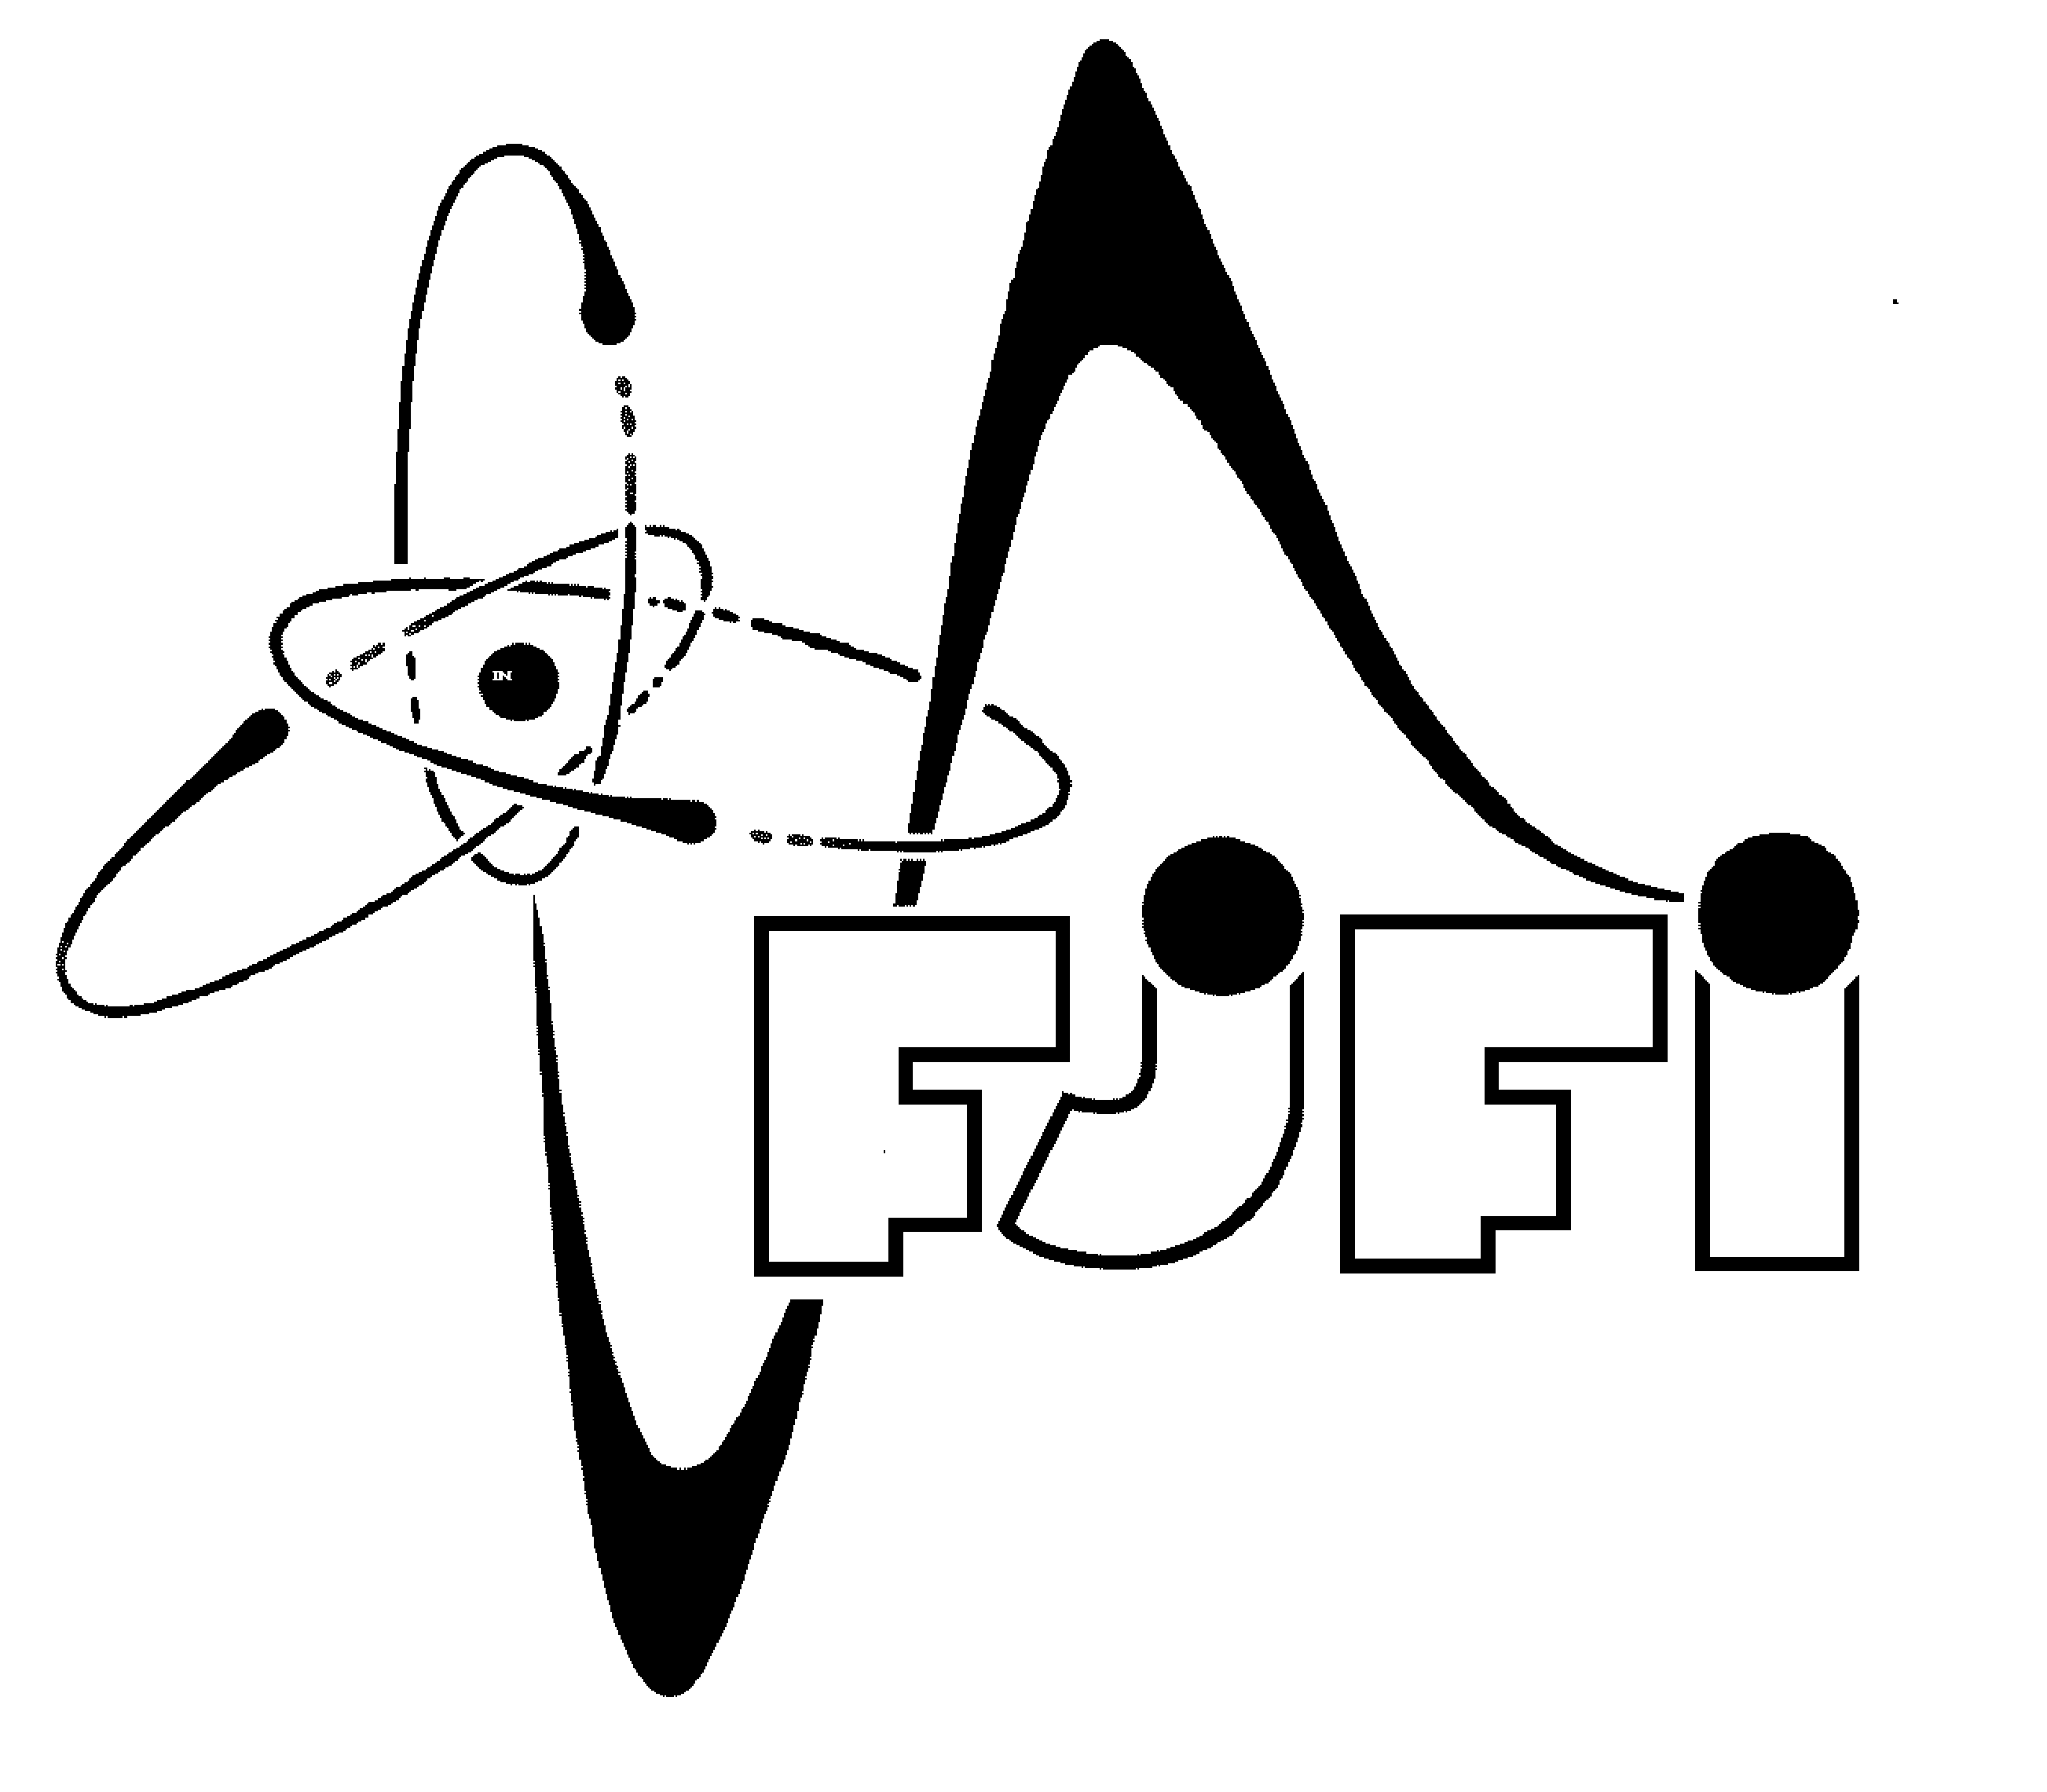
\includegraphics[width=3cm,height=3cm,keepaspectratio]{images/titlepage/fjfi}
	\end{minipage}

	\vspace{3.3cm}

	\setstretch{1.75}\textbf{\huge Název práce česky název práce česky název práce česky název práce česky}
	\vspace{1.1cm}

	\textenglish{\textbf{\huge Title of the Work in English Title of the Work in English Title of the Work in English}}
	\vspace{1.7cm}

	{\large Bakalářská práce}
\end{center}

\vfill

\begin{list}{}{
	\settowidth{\labelwidth}{MMMMMMMMM}
	\setlength{\leftmargin}{\labelwidth}
	\renewcommand{\makelabel}[1]{#1\hfil}}
	\item [{Autor:}] \textbf{Jméno Autora}
	\item [{Vedoucí práce:}] \textbf{prof. Ing. Jméno Školitele, DrSc.}
	\item [{Konzultant:}] \textbf{doc. RNDr. Jméno Konzultanta, CSc. }(pouze pokud konzultant byl jmenován.)
	\item [{Akademický rok:}] 2016/2017
\end{list}

\newpage

\null\newpage

\null\vfill
\begin{center}
	- Zadání práce -
\par\end{center}
\vfill

\newpage

\null\vfill
\begin{center}
	- Zadání práce (zadní strana) -
\par\end{center}
\vfill

\newpage

\noindent \textit{\Large Poděkování:}

\noindent Chtěl bych zde poděkovat především svému školiteli ...................
za pečlivost, ochotu, vstřícnost a odborné i lidské zázemí při vedení
mé diplomové práce. Dále děkuji svému konzultantovi ................
za ................

\vfill

\noindent \textit{\Large Čestné prohlášení:}

\noindent Prohlašuji, že jsem tuto práci vypracoval samostatně a uvedl
jsem všechnu použitou literaturu.

\bigskip

\noindent V Praze dne \documentdate\hfill Jméno Autora

\vspace{2cm}

\newpage

\null\newpage

\begin{onehalfspace}
	\noindent \textit{Název práce:}

	\noindent \textbf{Název práce}
\end{onehalfspace}

\bigskip

\noindent \textit{Autor:} Jméno Autora

\bigskip

\noindent \textit{Obor:} Celý název oboru (nikoliv zkratka)

\bigskip

\noindent \textit{Zaměření:} Celý název zaměření (Pokud obor neobsahuje
zaměření, tuto řádku odstranit.)

\bigskip

\noindent \textit{Druh práce:} Bakalářská práce

\bigskip

\noindent \textit{Vedoucí práce:} prof. Ing. Jméno Školitele, DrSc.,
pracoviště školitele (název instituce, fakulty, katedry...)

\bigskip

\noindent \textit{Konzultant:} doc. RNDr. Jméno Konzultanta, CSc., pracoviště
konzultanta. Pouze pokud konzultant byl jmenován.

\bigskip

\noindent \textit{Abstrakt:} Abstrakt max. na 10 řádků. Abstrakt max.
na 10 řádků. Abstrakt max. na 10 řádků. Abstrakt max. na 10 řádků.
Abstrakt max. na 10 řádků. Abstrakt max. na 10 řádků. Abstrakt max.
na 10 řádků. Abstrakt max. na 10 řádků. Abstrakt max. na 10 řádků.
Abstrakt max. na 10 řádků. Abstrakt max. na 10 řádků. Abstrakt max.
na 10 řádků. Abstrakt max. na 10 řádků. Abstrakt max. na 10 řádků.
Abstrakt max. na 10 řádků. Abstrakt max. na 10 řádků. Abstrakt max.
na 10 řádků. Abstrakt max. na 10 řádků. Abstrakt max. na 10 řádků.
Abstrakt max. na 10 řádků. Abstrakt max. na 10 řádků. Abstrakt max.
na 10 řádků. Abstrakt max. na 10 řádků. Abstrakt max. na 10 řádků.
Abstrakt max. na 10 řádků. Abstrakt max. na 10 řádků. Abstrakt max.
na 10 řádků. Abstrakt max. na 10 řádků. Abstrakt max. na 10 řádků. 

\bigskip

\noindent \textit{Klíčová slova:} klíčová slova (nebo výrazy) seřazená
podle abecedy a oddělená čárkou

\vfill

\begin{english}
	\begin{onehalfspace}
		\noindent \textit{Title:}

		\noindent \textbf{Title of the Work}
	\end{onehalfspace}

	\bigskip

	\noindent \textit{Author:} Author's Name

	\bigskip

	\noindent \textit{Abstract:} Max. 10 lines of English abstract text.
	Max. 10 lines of English abstract text. Max. 10 lines of English abstract
	text. Max. 10 lines of English abstract text. Max. 10 lines of English
	abstract text. Max. 10 lines of English abstract text. Max. 10 lines
	of English abstract text. Max. 10 lines of English abstract text.
	Max. 10 lines of English abstract text. Max. 10 lines of English abstract
	text. Max. 10 lines of English abstract text. Max. 10 lines of English
	abstract text. Max. 10 lines of English abstract text. Max. 10 lines
	of English abstract text. Max. 10 lines of English abstract text.
	Max. 10 lines of English abstract text. Max. 10 lines \cite{Allen-Cahn} of English abstract
	text. Max. 10 lines of English abstract text. Max. 10 lines of English
	abstract text. Max. 10 lines of English abstract text. Max. 10 lines
	of English abstract text. Max. 10 lines of English abstract text.
	Max. 10 lines of English abstract text. Max. 10 lines of English abstract
	text. Max. 10 lines of English abstract text.

	\bigskip

	\noindent \textit{Keywords:} keywords in alphabetical order separated
	by commas

\end{english}

\newpage

\null\newpage

\pagestyle{plain}

\tableofcontents

\newpage

\chapter*{Úvod}
\addcontentsline{toc}{chapter}{Úvod}

Text úvodu....

\chapter{Název první kapitoly}

\pagestyle{headings}

\chapter*{Závěr}
\addcontentsline{toc}{chapter}{Závěr}

\pagestyle{plain}

Text závěru....

\nocite{*}
\printbibliography[title=Literatura]

\end{document}
